\documentclass[conference]{IEEEtran}

\usepackage{cite}
\usepackage{amsmath,amssymb,amsfonts}
\usepackage{graphicx}
\usepackage{booktabs}
\usepackage{tabularx}
\usepackage{array}
\usepackage{placeins}
\usepackage{url}
\usepackage{xcolor}
\usepackage{tikz}
\usetikzlibrary{arrows.meta,positioning,shapes.geometric,fit}

\title{GPU-Accelerated Harris Corner Detection for Video Streams}

\author{%
\IEEEauthorblockN{Author Name(s)}
\IEEEauthorblockA{%
Department / Institution \\
City, Country \\
email@domain.com}
}

\begin{document}
\maketitle

\begin{abstract}
This report presents a CUDA-based implementation of the Harris corner detector for video processing. The manuscript summarizes the algorithmic background, related literature, project architecture, and CUDA-oriented processing pipeline in IEEE format. It also outlines the planned experimental methodology for evaluating resolution-dependent performance in video workloads.
\end{abstract}

\begin{IEEEkeywords}
Harris corner detection, CUDA, GPU acceleration, video processing, feature detection.
\end{IEEEkeywords}

\section{Introduction}
Corner detection is a core operation in computer vision pipelines including tracking, matching, motion analysis, and structure-from-motion. The Harris detector remains widely used due to its balance of computational cost, interpretability, and repeatability under moderate geometric and photometric variation. For high-frame-rate video, CPU implementations may become a bottleneck, motivating GPU acceleration.

This project implements a complete Harris pipeline with CUDA kernels for grayscale conversion, gradient estimation, second-moment matrix construction, Gaussian smoothing, response computation, and corner extraction. The implementation is integrated with OpenCV-based video input/output and frame-level visualization.

A practical and generic application scenario is \emph{real-time corner-enhanced video preprocessing for downstream vision modules}. In this setting, Harris corners are overlaid or exported as lightweight geometric cues before optional tracking, motion analysis, or scene understanding stages.

Performance behavior across different resolutions (480p, 720p, and 1080p) will be investigated and reported in the later experimental sections of this paper.

\section{Related Work (Literature Review)}

\subsection{Foundations of Corner Detection}
Harris and Stephens introduced an auto-correlation-based criterion that identifies points with significant intensity changes in two orthogonal directions~\cite{harris1988}. Their response measure, based on local gradient covariance, is computationally simple and has become a foundational building block for keypoint analysis.

Shi and Tomasi later proposed selecting features according to the minimum eigenvalue of the second-moment matrix~\cite{shi1994}, improving practical tracking stability for many scenes. In practice, Harris and Shi--Tomasi are often treated as neighboring methods on the same formulation family.

\subsection{Scale and Invariance-Oriented Detectors}
SIFT introduced robust scale-space keypoint detection and high-dimensional descriptors with strong matching performance under scale and rotation transformations~\cite{lowe2004}. SURF then targeted lower computational cost through approximations based on integral images~\cite{bay2008}.

These methods generally improve invariance and matching quality, but they can be heavier than Harris when the objective is low-latency detection in fixed or mildly varying imaging conditions.

\subsection{Real-Time Feature Alternatives}
ORB combines oriented FAST detection with rotated BRIEF descriptors and is widely used in real-time visual SLAM and embedded vision contexts~\cite{rublee2011}. Compared with Harris-based designs, ORB can provide strong runtime efficiency while trading off some sensitivity characteristics and descriptor assumptions.

\subsection{GPU Vision Context}
GPU execution is well-suited to this pipeline because its core stages (gradient computation, smoothing, and response evaluation) are data-parallel at the pixel level. Since each output depends on local neighborhoods with limited inter-pixel dependency, Harris is a natural candidate for CUDA optimization in streaming video workloads.

In summary, prior methods motivate different trade-offs between invariance, descriptor richness, and runtime. For this project, Harris is selected as a practical detector for frame-wise CUDA acceleration where low-latency corner extraction is prioritized over heavy descriptor computation.

\subsection{Literature Comparison with This Project}
Table~\ref{tab:lit-comparison} summarizes representative differences between foundational studies and the current project implementation.

\begin{table*}[t]
\caption{Literature comparison and positioning of the current CUDA Harris project}
\label{tab:lit-comparison}
\centering
\small
\begin{tabularx}{\textwidth}{>{\raggedright\arraybackslash}p{0.20\textwidth} >{\raggedright\arraybackslash}p{0.21\textwidth} >{\raggedright\arraybackslash}p{0.23\textwidth} >{\raggedright\arraybackslash}p{0.28\textwidth}}
\toprule
\textbf{Study / Method} & \textbf{Primary focus} & \textbf{Typical trade-off} & \textbf{Relation to this project} \\
\midrule
Harris--Stephens~\cite{harris1988} & Corner response from second-moment structure tensor. & Good efficiency and interpretability; limited scale invariance. & Core mathematical basis used in our CUDA frame pipeline. \\
Shi--Tomasi~\cite{shi1994} & Tracking-oriented corner quality criterion (minimum eigenvalue). & Often stable for tracking; still classical local-feature assumptions. & Alternative corner scoring reference; could be used as an ablation baseline. \\
SIFT~\cite{lowe2004} & Scale-invariant keypoint detection + high-dimensional descriptors. & Strong robustness, but heavier computation and descriptor cost. & Included as a robustness-oriented reference; not selected for low-latency target. \\
SURF~\cite{bay2008} & Faster approximation to SIFT using integral-image ideas. & Better speed than SIFT; still descriptor-heavy relative to Harris-only detection. & Useful comparison for speed/robustness balance, but not as lightweight as Harris response-only pipeline. \\
ORB~\cite{rublee2011} & Real-time oriented detector+binary descriptor. & Very fast matching pipeline; different detector/descriptor design goal. & Runtime-efficient alternative for future comparison; current project focuses on CUDA Harris response stages. \\
\textbf{This project (CUDA Harris)} & GPU-accelerated frame-wise Harris corner extraction for video. & Prioritizes detector throughput and modular kernel decomposition over descriptor invariance. & Targets resolution-dependent real-time behavior and straightforward integration into preprocessing workflows. \\
\bottomrule
\end{tabularx}
\end{table*}

The comparison in Table~\ref{tab:lit-comparison} highlights that the selected project direction emphasizes efficient detector-stage acceleration rather than descriptor-heavy matching. This positioning is aligned with the practical objective of frame-wise corner extraction on video streams, where deterministic execution flow and kernel modularity are prioritized. Based on this context, the next section details how the repository and CUDA modules are organized to support this implementation strategy.

\FloatBarrier
\section{System and Project Structure}

\subsection{Repository-Level Organization}
The repository is structured around kernel-by-kernel decomposition, with interface headers in \texttt{include/} and CUDA implementation files in \texttt{src/}. The entry point coordinates video decoding, per-frame GPU processing, and output encoding. This separation improves maintainability and enables independent profiling of each computational stage.

\begin{figure}[t]
\centering
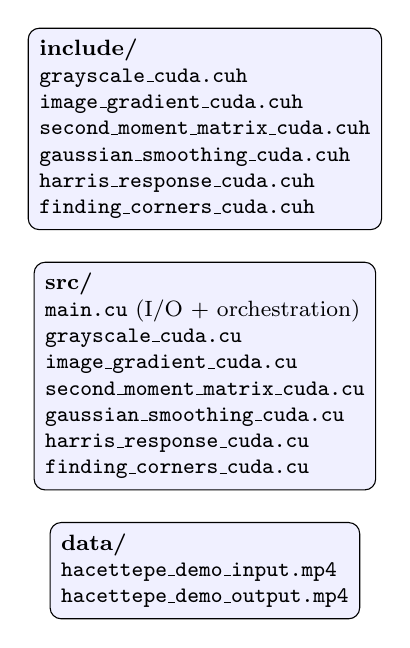
\begin{tikzpicture}[
node distance=4mm,
folder/.style={draw, rounded corners, fill=blue!6, align=left, font=\footnotesize, inner sep=4pt}
]
\node[folder] (inc) {\textbf{include/}\\
\texttt{grayscale\_cuda.cuh}\\
\texttt{image\_gradient\_cuda.cuh}\\
\texttt{second\_moment\_matrix\_cuda.cuh}\\
\texttt{gaussian\_smoothing\_cuda.cuh}\\
\texttt{harris\_response\_cuda.cuh}\\
\texttt{finding\_corners\_cuda.cuh}};
\node[folder, below=of inc] (src) {\textbf{src/}\\
\texttt{main.cu} (I/O + orchestration)\\
\texttt{grayscale\_cuda.cu}\\
\texttt{image\_gradient\_cuda.cu}\\
\texttt{second\_moment\_matrix\_cuda.cu}\\
\texttt{gaussian\_smoothing\_cuda.cu}\\
\texttt{harris\_response\_cuda.cu}\\
\texttt{finding\_corners\_cuda.cu}};
\node[folder, below=of src] (data) {\textbf{data/}\\
\texttt{hacettepe\_demo\_input.mp4}\\
\texttt{hacettepe\_demo\_output.mp4}};
\end{tikzpicture}
\caption{Project/module structure used in the CUDA Harris pipeline implementation.}
\label{fig:project-structure}
\end{figure}

\subsection{Execution Pipeline}
The video stream is first decoded into an ordered sequence of individual frames using host-side video I/O. Each decoded frame is treated as a standalone 2D image for GPU processing, while frame order is preserved to keep temporal consistency in the output video. After processing one frame, the corner-annotated result is returned to the output writer and the pipeline advances to the next frame.

Within each frame iteration, kernels are executed in a fixed dependency order and intermediate buffers are reused in device memory to reduce transfer overhead. Detailed per-kernel responsibilities are provided in the next subsection, while Figure~\ref{fig:pipeline} shows the stage-level flow.

\begin{figure*}[t]
\centering
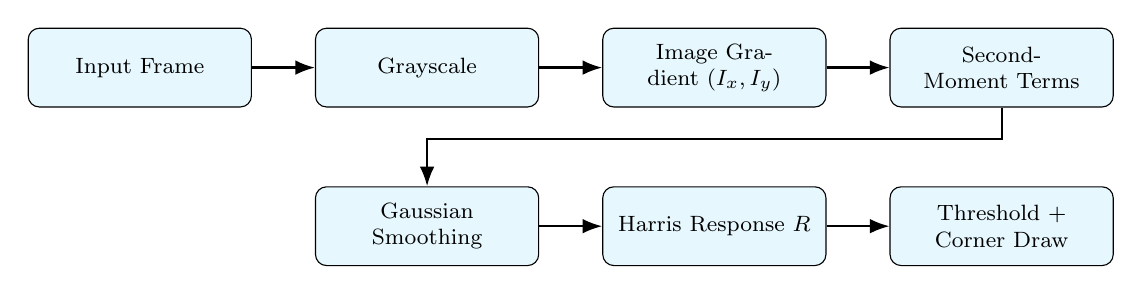
\begin{tikzpicture}[
procstep/.style={draw, rounded corners, minimum width=2.8cm, minimum height=1.0cm, align=center, fill=cyan!10, font=\footnotesize, text width=2.6cm},
arr/.style={-{Latex[length=2.5mm]}, thick}
]
% Top row
\node[procstep] (in) {Input Frame};
\node[procstep, right=8mm of in] (gray) {Grayscale};
\node[procstep, right=8mm of gray] (grad) {Image Gradient ($I_x, I_y$)};
\node[procstep, right=8mm of grad] (mom) {Second-Moment Terms};

% Bottom row
\node[procstep, below=10mm of gray] (gauss) {Gaussian Smoothing};
\node[procstep, right=8mm of gauss] (resp) {Harris Response $R$};
\node[procstep, right=8mm of resp] (corn) {Threshold + Corner Draw};

% Flow arrows
\draw[arr] (in) -- (gray);
\draw[arr] (gray) -- (grad);
\draw[arr] (grad) -- (mom);
\draw[arr] (mom.south) -- ++(0,-4mm) -| (gauss.north);
\draw[arr] (gauss) -- (resp);
\draw[arr] (resp) -- (corn);
\end{tikzpicture}
\caption{Frame-wise CUDA processing flow from input frame to corner-annotated output (two-row stage layout).}
\label{fig:pipeline}
\end{figure*}

\subsection{Kernel Responsibilities}
The following kernel-level descriptions define the functional responsibility of each CUDA module in the end-to-end Harris processing pipeline.

\subsubsection{\texttt{grayscale\_cuda.cu}}
Converts input color frames to single-channel intensity values used by all downstream operations. This stage standardizes pixel representation, reduces memory bandwidth for subsequent kernels, and ensures derivative operators work on a consistent luminance domain rather than three independent color channels.

\subsubsection{\texttt{image\_gradient\_cuda.cu}}
Computes horizontal and vertical image derivatives ($I_x$ and $I_y$), which form the basis of local structure analysis. In this project, Sobel filters are used for derivative estimation in both directions. The kernel maps one thread per pixel and applies local finite-difference style operations, producing gradient tensors that are consumed directly by second-moment computation.

\subsubsection{\texttt{second\_moment\_matrix\_cuda.cu}}
Builds per-pixel second-moment terms ($I_x^2$, $I_y^2$, and $I_x I_y$) before spatial smoothing. These quantities represent local directional energy and correlation, and they are stored in dedicated buffers to preserve precision through the subsequent smoothing stage.

\subsubsection{\texttt{gaussian\_smoothing\_cuda.cu}}
Applies Gaussian filtering to second-moment terms to stabilize neighborhood statistics and reduce noise sensitivity. By aggregating local evidence, this stage suppresses spurious gradient fluctuations and improves the numerical stability of the later Harris response evaluation.

\subsubsection{\texttt{harris\_response\_cuda.cu}}
Evaluates the Harris response function $R=\det(M)-k(\mathrm{trace}(M))^2$ for each pixel. The kernel combines smoothed tensor components into a scalar corner-strength map, where strong positive responses indicate candidate corner structures.

\subsubsection{\texttt{finding\_corners\_cuda.cu}}
Applies thresholding and corner-selection logic, then prepares output corner annotations. This stage filters weak responses, keeps salient locations, and writes overlay-ready coordinates/intensity cues for frame visualization in the final output stream.

\section{Method Details}
\subsection{Mathematical Formulation}
Let an input RGB frame be denoted by channels $R(x,y)$, $G(x,y)$, and $B(x,y)$. The grayscale conversion used before derivative computation is
\begin{equation}
I(x,y) = 0.299\,R(x,y) + 0.587\,G(x,y) + 0.114\,B(x,y).
\end{equation}

For filtering-oriented stages, padding is applied on the CPU side to create an extended image $\tilde{I}(x,y)$ so neighborhood reads remain valid at boundaries. Using this padded representation, derivative and smoothing operations follow standard local convolution forms:
\begin{equation}
I_x = K_x * \tilde{I}, \qquad I_y = K_y * \tilde{I},
\end{equation}
where $K_x$ and $K_y$ are Sobel derivative kernels (applied in horizontal and vertical directions, respectively) and $*$ denotes convolution. In this implementation, both Sobel and Gaussian filtering use $3\times3$ masks; these neighborhood operators require more computation than point-wise transforms, while still remaining lighter than larger filtering windows.

The second-moment matrix is then computed as
\begin{equation}
M = \begin{bmatrix}
G_\sigma * I_x^2 & G_\sigma * I_x I_y \\
G_\sigma * I_x I_y & G_\sigma * I_y^2
\end{bmatrix},
\end{equation}
where $G_\sigma$ is Gaussian smoothing. The Harris response is
\begin{equation}
R = \det(M) - k\, (\mathrm{trace}(M))^2.
\end{equation}
Pixels with large positive $R$ are interpreted as corners.

\subsection{Implementation Notes}
The staged decomposition in this project favors debuggability and selective optimization. The use of $3\times3$ Sobel and $3\times3$ Gaussian filters provides a practical balance between edge/corner quality and computational load. First, kernels can be validated independently against CPU-side references. Second, performance counters can be captured per stage to identify bottlenecks (e.g., memory bandwidth pressure in smoothing versus arithmetic intensity in response calculation). Third, parameter sweeps can be localized to one stage (e.g., Gaussian window size) without destabilizing the full pipeline. The implementation also applies CPU-side padding before filtering kernels to reduce boundary-branch complexity inside GPU convolutions.

\textbf{Missing information to add:}
\begin{itemize}
    \item Numerical settings for $k$, Gaussian kernel size, and threshold.
    \item Border handling policy (replicate, reflect, clamp, etc.).
    \item Non-maximum suppression details (window size, tie-breaking).
    \item Exact device-memory layout and per-stage buffer reuse policy.
    \item Final numeric launch parameters used in experiments (block width/height and resulting grid dimensions).
    \item Measured stream-overlap benefit for non-filtering kernels (if reported in results).
\end{itemize}

\section{Experimental Plan (Results Pending)}
This section is intentionally designed to be completed after profiling and quality experiments.

\subsection{Planned Metrics}
\begin{itemize}
    \item Runtime per frame (ms) and throughput (FPS) at multiple resolutions.
    \item End-to-end speedup versus a CPU baseline implementation.
    \item Temporal consistency of detected corner counts.
    \item Optional repeatability/localization quality on benchmark image pairs.
\end{itemize}

\subsection{Planned Comparisons}
\begin{itemize}
    \item Harris GPU vs Harris CPU (same thresholds and smoothing settings).
    \item Harris GPU vs ORB/FAST detection runtime (if integration is available).
    \item Sensitivity to scene texture, motion blur, and illumination changes.
\end{itemize}

\subsection{Planned Ablations}
\begin{itemize}
    \item Gaussian kernel size impact on noise robustness vs runtime.
    \item Harris threshold impact on precision-recall-like behavior.
    \item Resolution scaling behavior and memory footprint trends.
\end{itemize}

\textbf{Missing information to add:}
\begin{itemize}
    \item GPU and CPU hardware/software configuration table.
    \item Dataset/video characteristics (resolution, duration, scene classes).
    \item Reproducible protocol (warm-up, run count, averaging, variance reporting).
    \item Whether timings are kernel-only or include host-device transfer and rendering.
\end{itemize}

\section{Threats to Validity and Limitations}
Potential limitations include sensitivity to weak-texture regions, threshold dependence, and possible corner instability under severe blur or abrupt lighting changes. Experimental validity may also be affected by non-deterministic GPU scheduling noise, video codec variability, and inconsistent CPU frequency scaling.

\textbf{Missing information to add:}
\begin{itemize}
    \item Any observed failure modes from your demo videos.
    \item Statistical confidence intervals for reported performance values.
\end{itemize}

\section{Conclusion and Next Steps}
This draft now provides a more complete 6--8 page report foundation by expanding literature coverage, detailing project structure, and adding figures that clarify module layout and frame processing flow. The next revision should integrate measured results and comparative analysis to support final technical claims.

\textbf{Missing information to add:}
\begin{itemize}
    \item Final quantitative conclusions from experiments.
    \item Optimization recommendations derived from profiling.
    \item Priority roadmap for further acceleration or robustness improvements.
\end{itemize}

\bibliographystyle{IEEEtran}
\bibliography{references}

\end{document}
